\section*{Microeconomics Midterm 2011 / 12}

{
\subsection*{Schmidt}

\subsubsection*{Exercise 1}

\begin{enumerate}[label=(\alph*)]
{\item 
As all bundles are different, we need to check for affordability of each bundle under each price-wealth-situation.
As we see in the table, whenever $p^t \times\left(p^{t^{\prime}}, w^{t^{\prime}}\right) \leq w^t$ we have $p^{t^{\prime}} \times\left(p^t, \omega^t\right)>\omega^{t^t}$, and WA holds.

\begin{table}[h!]
    \centering
    \begin{tabular}{c|c|c|c|c}
        Situation & Bundle & Expenditure & Compare & Conclusion \\\hline
        at $\left(p^0, w^0\right)$ & $x^1$ & $p^0 x^1=96$ & $>w^0$ & $x^1$ not aff. \\
        & $x^2$ & $p^0 x^2=80$ & $<w^0$ & $x^2$ is aff. \\
        at $\left(p^1, w^1\right)$ & $x^0$ & $p^1 x^0=33$ & $<w^1$ & $x^1$ is aff. \\
        & $x^2$ & $p^1 x^2=39$ & $>w^1$ & $x^2$ not aff. \\
        at $\left(p^2, w^2\right)$ & $x^0$ & $p^2 x^0=52$ & $>w^2$ & $x^1$ not aff. \\
        & $x^2$ & $p^1 x^2=48$ & $<w^2$ & $x^2$ is aff. \\
    \end{tabular}
\end{table}
}

{\item 
Whenever multiple bundles are affordable under are price-wealth-situation, we can make observations about revealed preference:

\begin{itemize}
    \item at $\left(p^0, w^0\right): x^0 \succ x^2$
    \item at $\left(p^1, w^1\right): x^1 \succ x^0$

    By transitivity we must have $x^1 \succ x^2$. But:
    \item at $\left(p^2, w^2\right): x^2 \succ x^1$
\end{itemize}

We have found a violation of transitivity.
}
\end{enumerate}
}

{
\subsubsection*{Exercise 2}

\begin{enumerate}[label=(\alph*)]
{\item
Apply Roy's identity:

\begin{align*}
    x_1(p,w) &= -\frac{\frac{\partial v(p w)}{\partial p_1}}{\frac{\partial v(p w)}{\partial w}} = -\frac{\frac{w}{p_1^2}}{\frac{1}{p_1} + \frac{1}{p_2}} = \frac{w}{p_1} \frac{1}{1+\frac{p_1}{p_2}}
\end{align*}
}
{\item
(1) Invert $v(p, w)$ to find $w$. At optimum we have $v(p, w)=u ; w=e(p, u)$:

\begin{align*}
    w & =v\left(p, w\right) \frac{1}{\frac{1}{p_1}+\frac{1}{p_2}}=v\left(p, w\right)\left[\frac{1}{p_1}+\frac{1}{p_2}\right]^{-1} \\
    \Longleftrightarrow e\left(p, u\right) & =u\left[\frac{1}{p_1}+\frac{1}{p_2}\right]^{-1}
\end{align*}

(2) Apply Shephard's Lemma:
\begin{align*}
    h_1(p, u) & =\frac{\partial e\left(p,u\right)}{\partial p_1}=u(-1)\left[\frac{1}{p_1}+\frac{1}{p_2}\right]^{-2}(-1) \frac{1}{p_1^2} \\
    & =u\left[1+\frac{p_1}{p_2}\right]^{-2}
\end{align*}
}
{\item 
Yes.

\begin{align*}
    x_1\left(\lambda p, \lambda w\right)=\frac{\lambda w}{\lambda p_1} \frac{1}{1+\frac{\lambda p_1}{\lambda p_2}}=\frac{w}{p_1} \frac{1}{1+\frac{p_1}{p_2}}=x_1\left(p, w\right)
\end{align*}
}
{\item 
Let $f(\cdot)$ be a monotonic transformation.
Then by Roy's identity:

\begin{align*}
    & \tilde{x}_l(p, w)=-\frac{\frac{\partial f(v(p, w))}{\partial p_l}}{\frac{\partial f(v(p,w))}{\partial w}} \quad \text { apply chain-rule } \\
    & =-\frac{\frac{\partial f\left(v\left(p, w\right)\right)}{\partial v\left(p, w\right)} \cdot \frac{\partial v\left(p, w\right)}{\partial p_l}}{\frac{\partial f\left(v\left(p, w\right)\right.}{\partial v(p, w)} \cdot \frac{\partial v\left(p, w\right)}{\partial w}} 
    =-\frac{\frac{\partial v\left(p, w\right)}{\partial p_l}}{\frac{\partial v(p, w)}{\partial w}}=x_l(p, w)
\end{align*}
}
\end{enumerate}
}

{
\subsubsection*{Exercise 3}

\begin{enumerate}[label=(\alph*)]
{\item
\underline{IF:}

\begin{align*}
    u(x) &= \alpha + \beta \left( -e^{-cx} \right) \\
    u^\prime(x) &= -c\beta \left( -e^{-cx} \right) \\
    u^{\prime\prime}(x) &= -c^2\beta \left( -e^{-cx} \right) \\
    r(x) &= -\frac{-c^2 \beta e^{-c x}}{c \beta e^{-c x}}=c
\end{align*}

\underline{ONLY IF:}

\begin{align*}
    & r(x)=-\frac{u^{\prime \prime}(x)}{u^{\prime}(x)}=-\frac{d \ln \left(u^{\prime}(x)\right)}{d x}=c \\
    & \int_{\underline{x}}^x \frac{d \ln\left(u^{\prime}(t)\right)}{d t} d t=-c \int_{\underline{x}}^x d t \\
    & \ln \left(u^{\prime}(x)\right)-\ln \left(u^{\prime}(\underline{x})\right)=-c(x-\underline{x}) \\
    & \frac{u^{\prime}(x)}{u^{\prime}(\underline{x})}=\exp (-c x) \exp (c \underline{x}) \\
    & \int_{\underline{x}}^x u^\prime(y) dy = \int_{\underline{x}}^x \exp (-c y) d t \exp (c \underline{x}) u^{\prime}(\underline{x}) \\
    & u(x)-u(\underline{x})=-\frac{1}{c}(\exp (-c x)-\exp (-c \underline{x})) \exp (c \underline{x}) u^{\prime}(\underline{x}) \\
    & u(x)=u(\underline{x})-\frac{1}{c}(\exp (-c x)-\exp (-c \underline{x})) \exp (c \underline{x}) u^{\prime}(\underline{x})
\end{align*}

By choosing $\alpha, \beta, c$ correctly, we can get:

\begin{align*}
    u(x)=\alpha-\beta \exp (-c x)
\end{align*}
}
{\item 
\begin{align*}
    \max _a E U(w-a+a z) = 
    \max _a \int-\exp (-c(w-a+a z)) d F(z)
\end{align*}

Obtain the FOC:

\begin{align*}
    \frac{\partial E U(\cdot)}{\partial a}=\int-\exp (-c(w-a+a z))(-c)(z-1) d F(z)  &\stackrel{!}{=} 0 \\
    c \int \exp (-c w) \exp (c a) \exp (-c a z)(z-1) d F(z) &=0 \\
    \underbrace{c \cdot \exp (-c w) \exp (c a)}_{\neq 0} \int \exp (-c a z)(z-1) d F(z) &=0 \\
    \int \exp (-\operatorname{caz})(z-1) d F(z) &=0
\end{align*}

The last line implicitly defines the optimal $\tilde{a}$ and it is independent of $w$.
}
\end{enumerate}
}

\newpage
{
\subsection*{Gottardi}

\subsubsection*{Exercise 1}

\begin{enumerate}[label=(\alph*)]
{\item 
Maximum production / consumption: $2 \cdot 8=16$
Maximum leisure : $8$

The blue triangle (incl. border) is feasible. The border is the set of PE allocations, described by

\begin{align*}
    c=16-2 e
\end{align*}

\begin{figure}[h!]
    \centering
    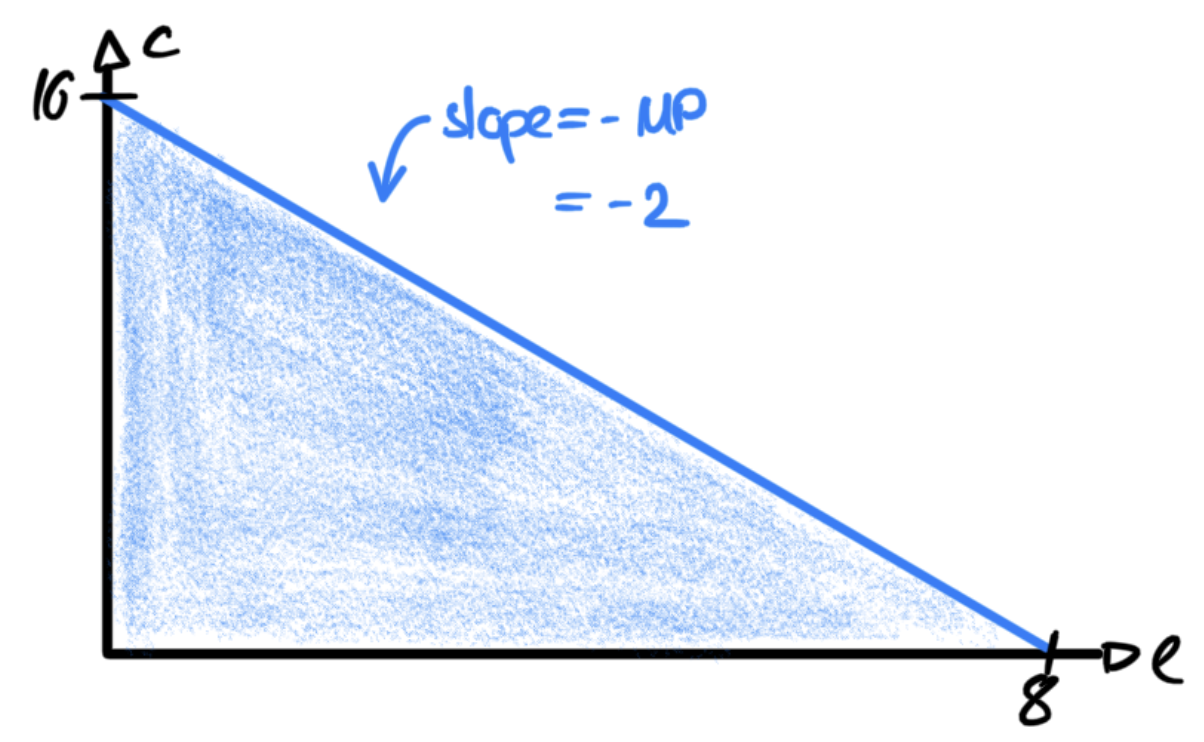
\includegraphics[width=0.75\linewidth]{images/2013_14_1.png}
\end{figure}
}
{\item 
\underline{Consumer Problem:}

\begin{align*}
    \max & c+l^{1 / 2} \\
    \text { s.t. } & p c=\omega[8-l]+\pi
\end{align*}

FOCs:

\begin{align*}
    1-\lambda p &= 0 \\
    \frac{1}{2} l^{-1 / 2}-\lambda w &= 0 \\
    \Longrightarrow\quad \frac{1}{2} l^{-1 / 2}&=\frac{w}{p} \\
    \Leftrightarrow\quad l&=\left(\frac{p}{w} \frac{1}{2}\right)^2
\end{align*}

\underline{Firm Problem:}

\begin{align*}
    \max _L p 2L-w L \Leftrightarrow \max _L L(2 p-w) \\
    L=\left\{\begin{array}{lll}
        \infty & \text { if } p/ w>1 / 2 \\
        \mathbb{R}^{+} & \text {if } p/ w=1 / 2 \\
        0 & \text { if } p/ w<1 / 2
    \end{array}\right.
\end{align*}

\underline{Market Clearing:}

\begin{align*}
    & c=y=2 L \\
    & l=8-L \\
    \Longrightarrow\quad & c=2(8-l)
\end{align*}

Since any price other than $1 / 2$ would lead to excess demand of one good or the other, set

\begin{align*}
    \frac{p}{w}=1 / 2 \longrightarrow l=\frac{1}{16} & \longrightarrow C=\frac{127}{8}=y \\
    & \longrightarrow L=\frac{127}{16}
\end{align*}

\underline{Competitive Equilibrium:}

\begin{align*}
    y=\frac{127}{8} ; L=\frac{127}{16} ; \frac{p}{w}=\frac{1}{2}
\end{align*}

\begin{figure}[h!]
    \centering
    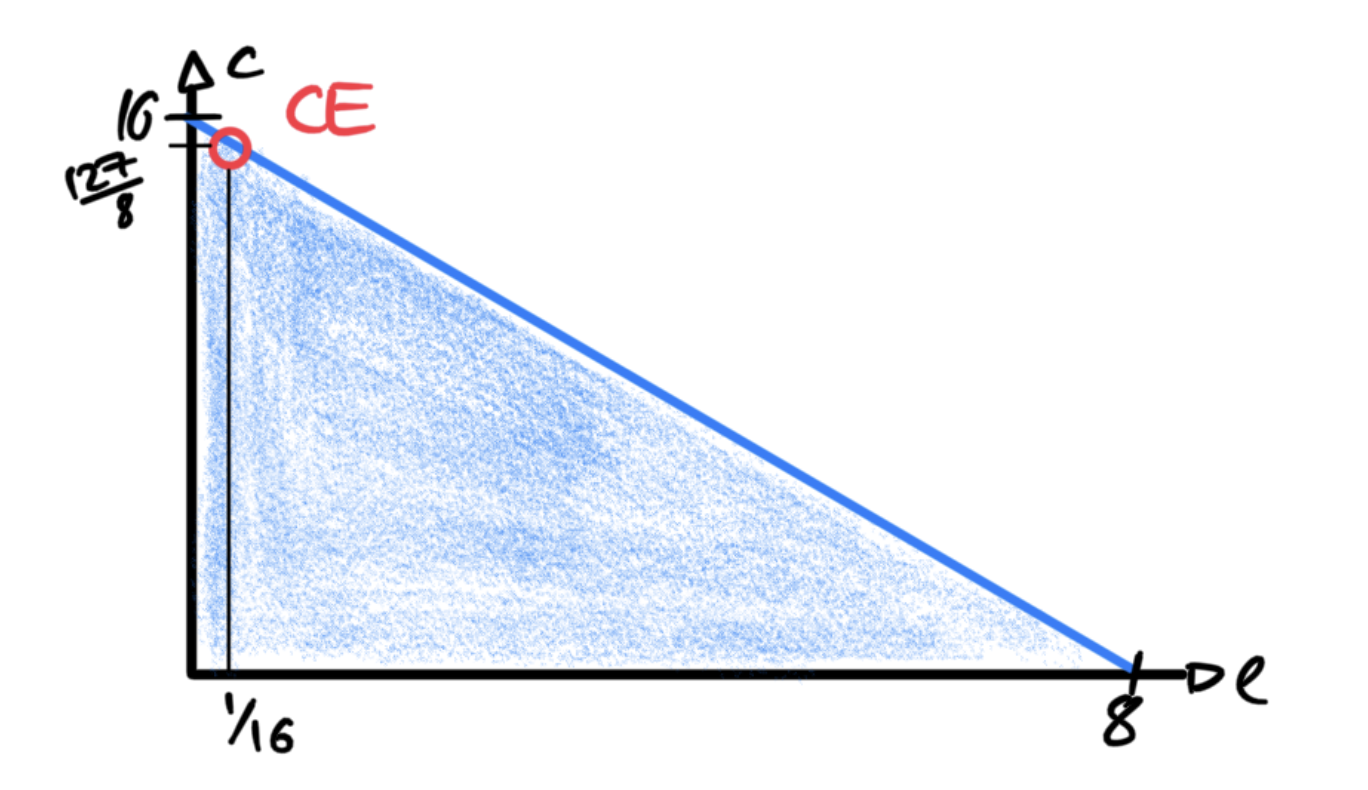
\includegraphics[width=0.75\linewidth]{images/2013_14_2.png}
\end{figure}
}
{\item 
This shifts the equilibrium along the PE allocations to more leisure and less consumption. 
Nothing changes for the firm. Thus: $\frac{p}{w} = \frac{1}{2}$ as before. For the consumer we now have $l=\left(\frac{p}{w}\right)^2=\frac{1}{4}=0.25$.
Thus:

\begin{align*}
    L = 8 - \frac{1}{4} = 7.75 \\
    c = y = 2L = 15.5
\end{align*}

Output decreases as the consumer wants to work less which decreases the input $L$ decreasing output.
}
\end{enumerate}
}
{
\subsubsection*{Exercise 2}

We need:
\begin{itemize}
    \item Convexity of preferences
    \item Continuity of aggregate demand
    \item as $p_l \rightarrow 0$ we have that $z_l>0$ and
    
    as $p_l \rightarrow \infty$ we have that $z_l<0$
\end{itemize}

Suppose continuity is violated. As we see $z_l = 0$ does not occur. Without market clearing, there is no CE.

\begin{figure}[h!]
    \centering
    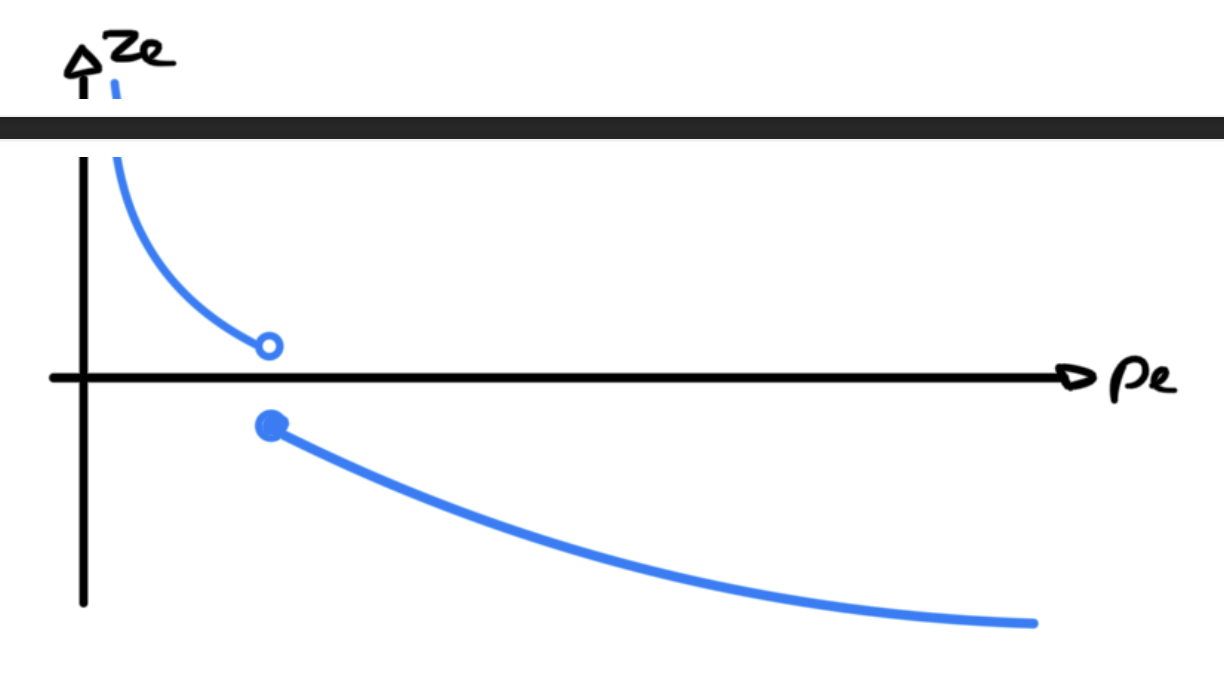
\includegraphics[width=0.75\linewidth]{images/2013_14_3.png}
    \caption{Ignore the horizontal line. It was created by accident when exporting the drawing from the iPad.}
\end{figure}
}
{
\subsubsection*{Exercise 3}

$w^h=(2,2)$

\begin{enumerate}[label=(\alph*)]
{\item 
\begin{align*}
    \text{at } t = 0: & q_1 \theta_1^h+q_2 \theta_2^h=0 \\
    \text{at } t = 1: & x^h(1)=2+\theta_1^h \\
    & x^h(2)=2+\theta_2^h
\end{align*}

Combine into one BC:

\begin{align*}
    q_1 \left[ x^h(1) -2\right] +q_2\left[x^h(2)-2\right]=0
\end{align*}

\underline{Consumer h:}

\begin{align*}
    & \max _{x^h(s)} \pi^h \ln \left(x^h(1)\right)+\left(1-\pi^h\right) \ln \left(x^h(2)\right) \\
    & \text{s.t. } q_1\left[x^h(1)-2\right]+q_2\left[x^h(2)-2\right]=0
\end{align*}

FOCs

\begin{align*}
    \pi^h \frac{1}{x^h(1)}-\lambda q_1&=0 \\
    (1-\pi^h) \frac{1}{x^h(2)}-\lambda q_2&=0 \\
    \Longrightarrow\quad \frac{\pi^h}{1-\pi^h} x^h(2) &= \frac{q_1}{q_2} x^h(1)
\end{align*}

Plug into BC:

\begin{align*}
    & \frac{\pi^h}{1-\pi^h} x^h(2)-2 \frac{q_1}{q_2}+x^h(2)-2=0 \\
    & x^h(2)\left[\frac{\pi^h}{1-\pi^h}+1\right]=2\left(1+\frac{q_1}{q_2}\right) \\
    & x^h(2)=2\left(1+\frac{q_1}{q_2}\right)\left(1-\pi^h\right)
\end{align*}

\underline{Market Clearing:}

\begin{align*}
    x^1(2)+x^2(2)=4 \\
    2\left(1+\frac{q_1}{q_2}\right)\left[1-\pi^1+1-\pi^2\right]=4 \tag{I} \\
    \stackrel{\pi^1=\pi^2}{\Longrightarrow} 4\left(1+\frac{a_1}{q_2}\right)(1-\pi)=4 \\
    \Longrightarrow \frac{q_1}{q_2}=\frac{1}{1-\pi}-1=\frac{\pi}{1-\pi}
\end{align*}

Thus: $x^1(2)=x^1(1) ; x^2(1)=x^2(2)$ which I plug into BC:

\begin{align*}
    \left(q_1+q_2\right)\left[x^h(s)-2\right]=0 \\
    \Longleftrightarrow \quad x^h(s)=2 \quad \forall s, h
\end{align*}

\underline{Competitive Equilibrium:}

\begin{align*}
    \left(x^1(1), x^1(2)\right) & =(2,2) \\
    \left(x^2(1), x^2(2)\right) & =(2,2) \\
    \frac{q_1}{q_2} & =\frac{\pi}{1-\pi}
\end{align*}

There is no trade. Reason being that the consumers are perfectly identical. There is no gain from exchanging anything.
}
{\item 
Everything up to (I) is identical. From there:

\begin{align*}
    \left(1+\frac{q_1}{q_2}\right)\left(2-\pi^1-\pi^2\right) & =2 \\
    \Longrightarrow \frac{q_1}{q_2} =\frac{2}{2-\pi^{1}-\pi^2}-1 = \frac{\pi^1+\pi^2}{\left(1-\pi^1\right)+\left(1-\pi^2\right)} &= 1
\end{align*}

Therefore we find

\begin{align*}
    \left(x^1(1), x^1(2)\right) &= (1,3) \\
    \left(x^2(1), x^2(2)\right) &= (3,1)
\end{align*}

Agent 1 increases (decreases) state 1 (2) consumption. Vice versa for agent 2. I.e. agent 1 buys asset 1 because she believes state 1 to be more likely. Thus it is optimal for her to insure against being poor in that state. Agent 2 does the opposite. Clearly there is trade through the Arrow securities.
}
\end{enumerate}
}
